\section{Introduction}
\label{sec:introduction}

% state the learning objective
\paragraph{} 
The objective of this laboratory assignment is to study an RC circuit containing a voltage source $v_S$ (defined by the fllowing sinusoidal equation: $v_s (t) = V_s u(−t) + sin(2 \pi ft)u(t) $), a current-controlled voltage source $V_D$, a voltage-controlled current source $I_B$ and a capacitor $C$ connected to different fixed value resistors $R_1$, $R_2$, $R_3$, $R_4$, $R_5$, $R_6$ and $R_7$.
The circuit can be seen in Figure~\ref{fig:circuit}.


\paragraph{}
In Section~\ref{sec:theoretical}, a theoretical introduction is made in order to contextualize all the main principles that sustain our analysis of the circuit. This circuit is carefully analysed according to six different theoretical analysis topics, presented in Section~\ref{sec:analysis}, where the results are obtained in GNU Octave. Also, in Section~\ref{sec:simulation}, the circuit is analysed by simulation through the use of NGSpice to simulate the electric circuit behaviour. The results of the simulation of Section~\ref{sec:simulation} are then compared to the theoretical results obtained in Section~\ref{sec:analysis} and the comparative results are expressed in Section~\ref{sec:erroranalysis}. The conclusions of this study are outlined in the final part of the report, in Section~\ref{sec:conclusion}.


\begin{figure}[h] \centering
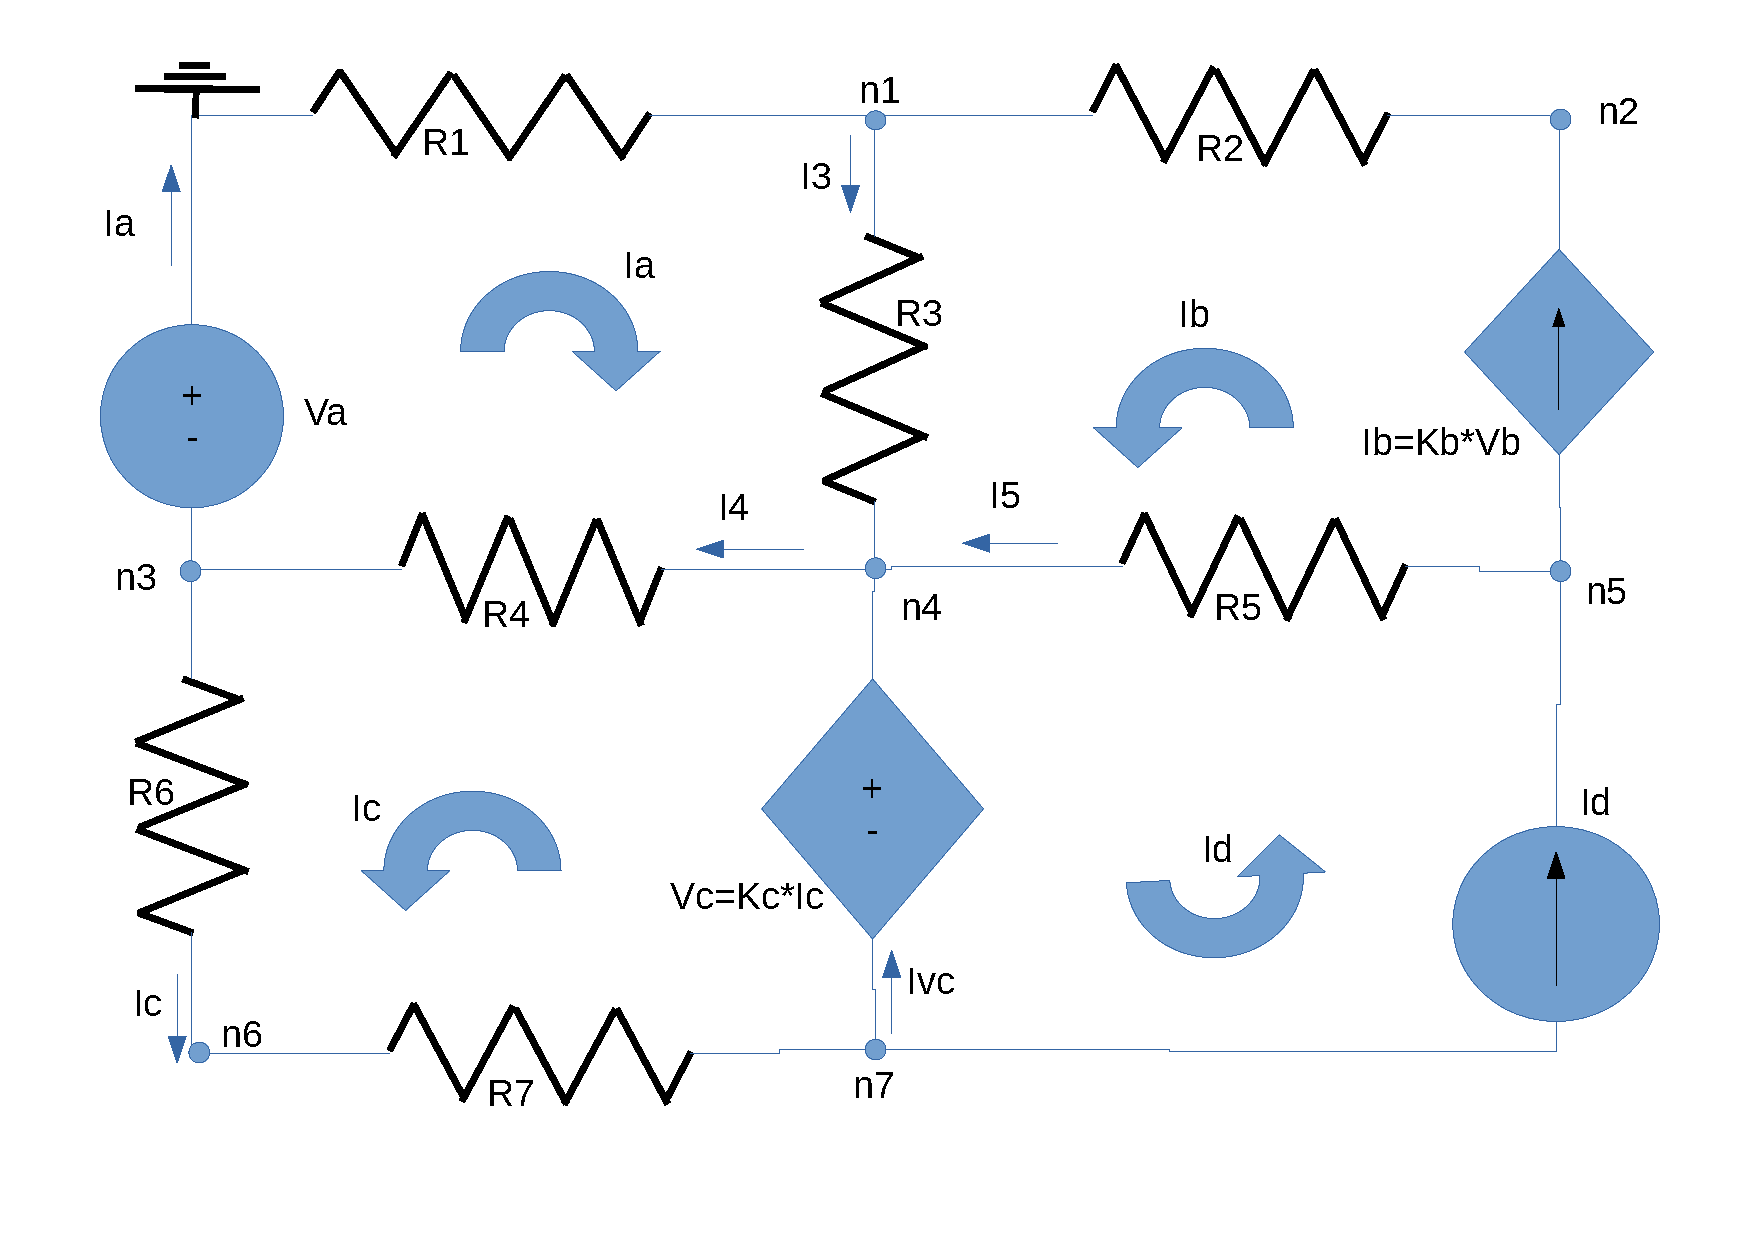
\includegraphics[width=0.4\linewidth]{circuit.pdf}
\caption{Second laboratory circuit.}
\label{fig:circuit}
\end{figure}

